\documentclass[tikz,convert={outfile=\jobname.pdf}]{standalone}
%\usetikzlibrary{...}% tikz package already loaded by 'tikz' option
\usepackage{makeshape}
\usepackage{flowchart}
\usetikzlibrary{arrows}

\begin{document}
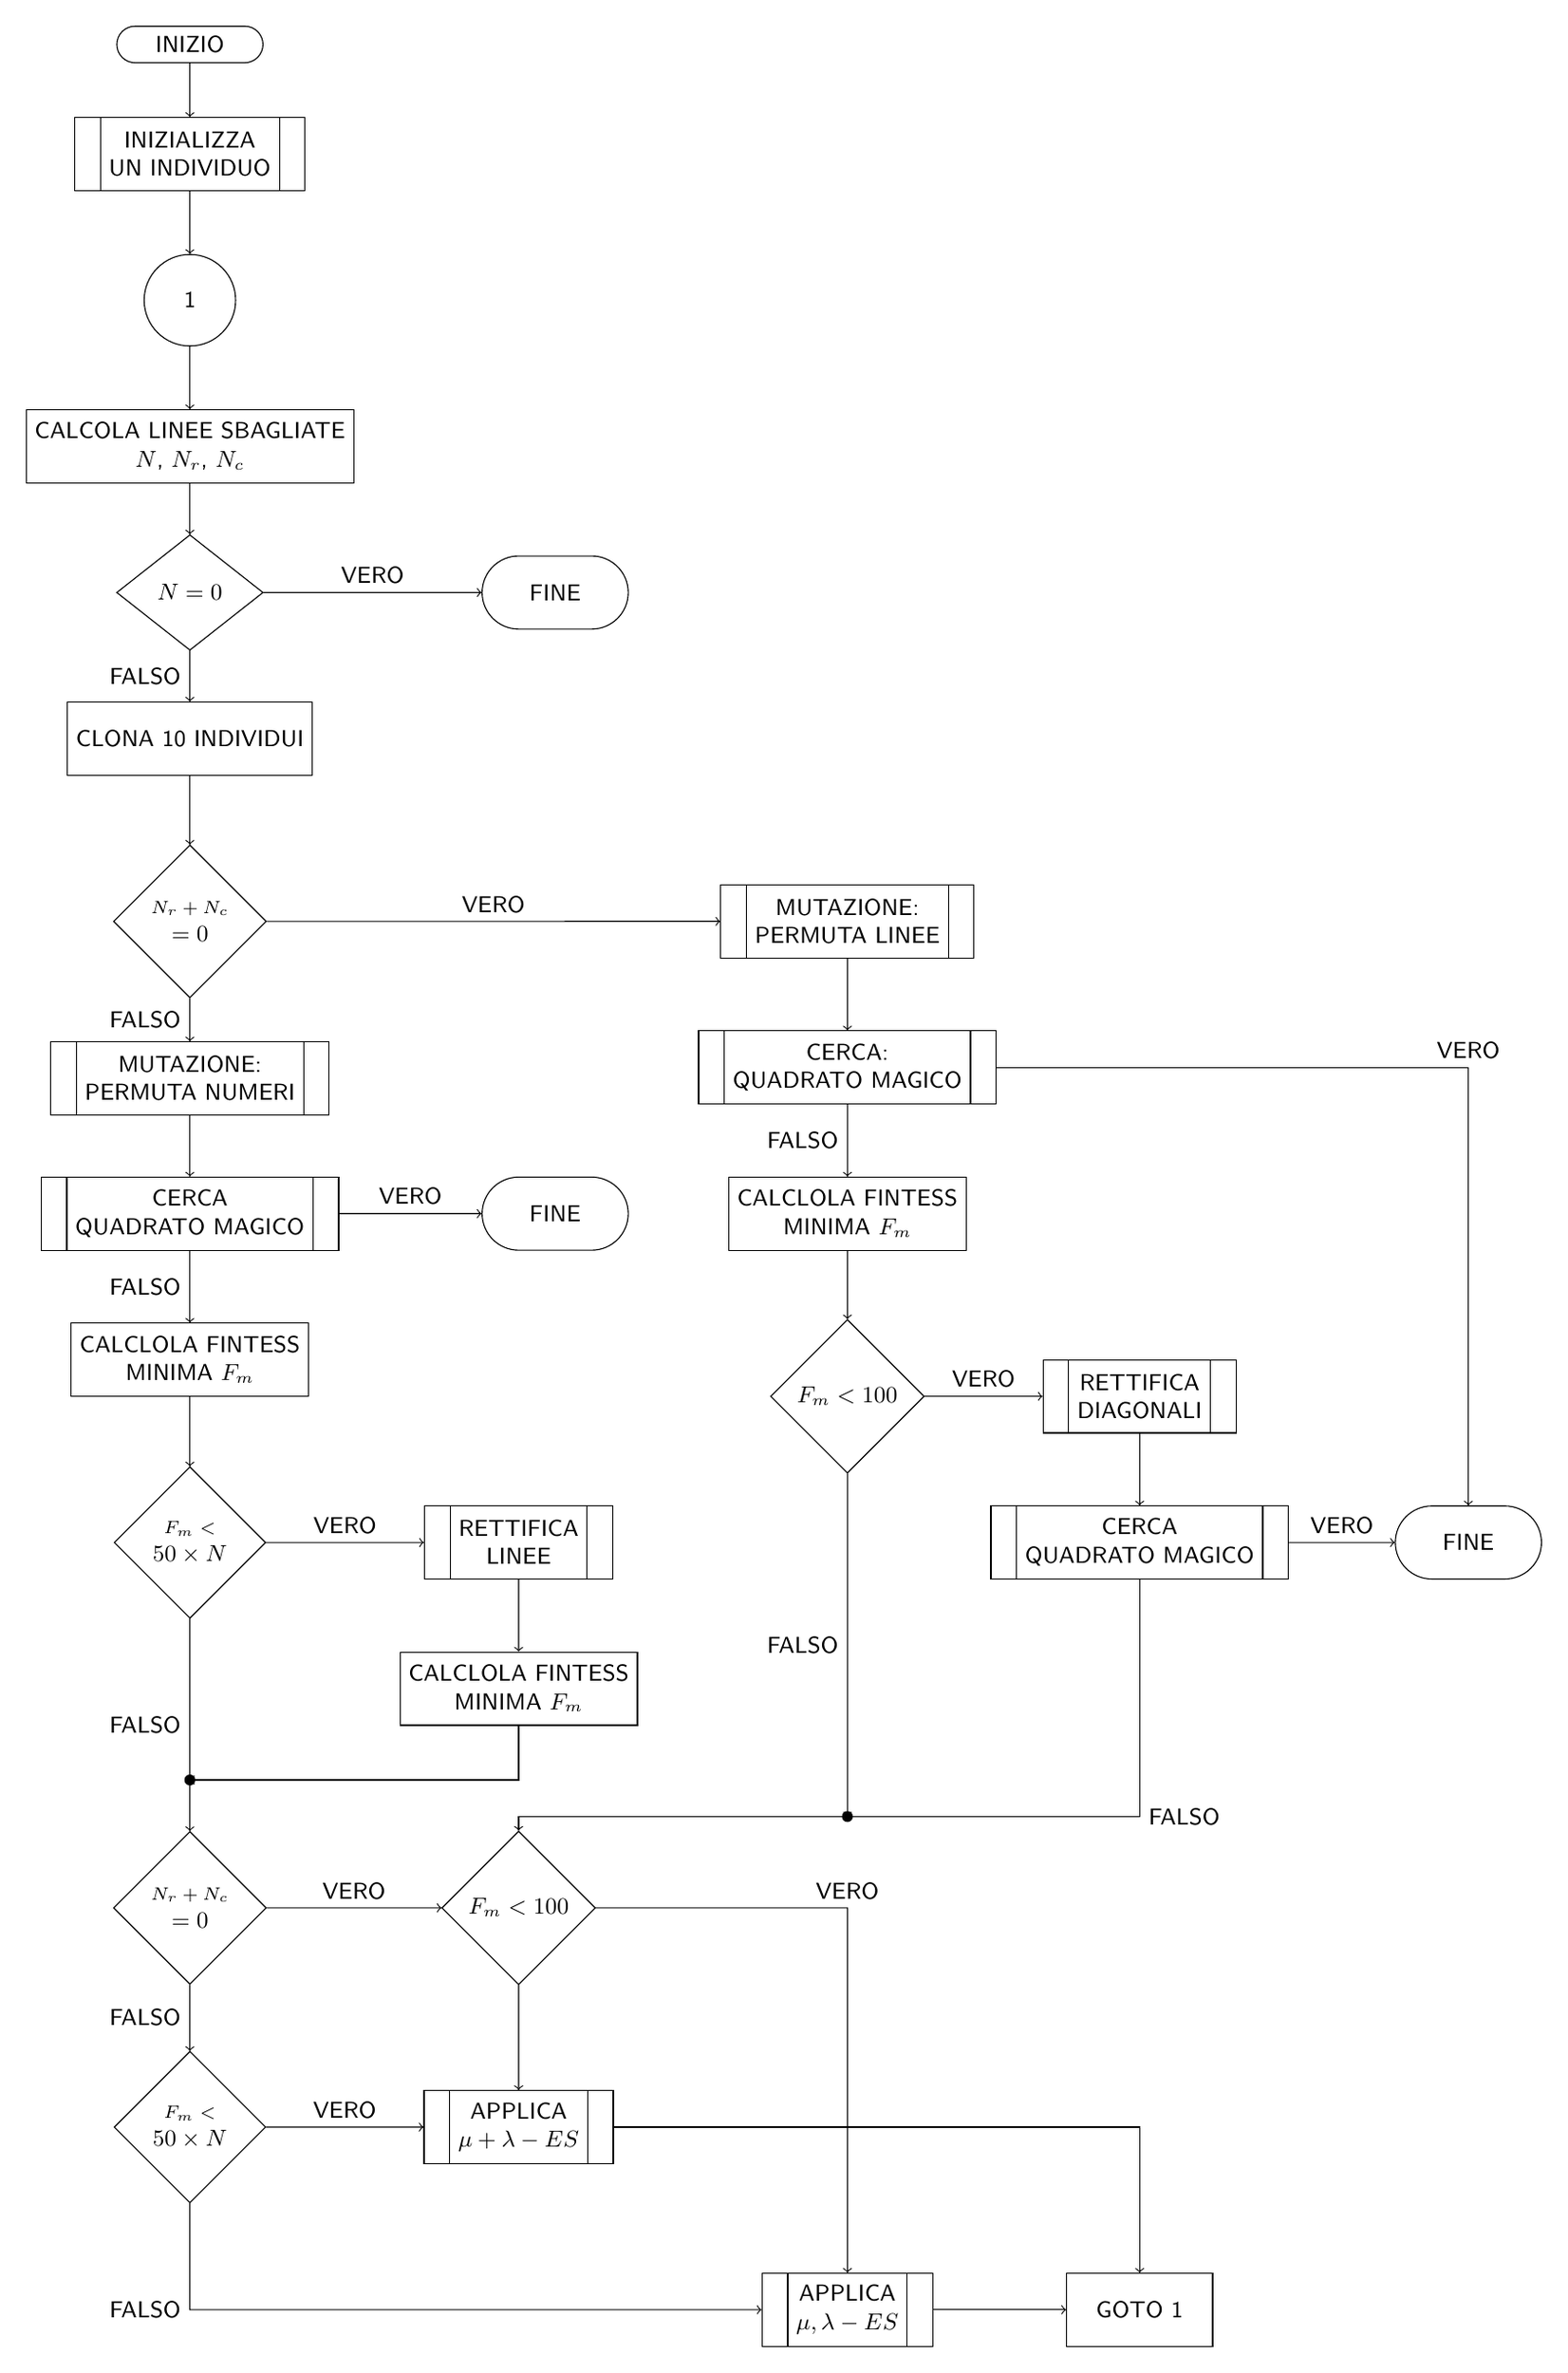
\begin{tikzpicture}[font={\sf \small}]
\def\smbwd{2cm}
\node (terminal1) at (0,2) [draw, terminal,
minimum width=\smbwd,
minimum height=0.5cm] {INIZIO};
\node (predproc1) at (0,0.5) [draw, predproc, align=center,
minimum width=\smbwd,
minimum height=1cm] {INIZIALIZZA\\ UN INDIVIDUO};
\node[draw, circle,inner sep=10] (1) at (0, -1.5) {1};
\node (calcola1) at (0, -3.5) [draw, process, align=center,
minimum width=\smbwd,
minimum height=1cm] {CALCOLA LINEE SBAGLIATE\\ $ N $, $ N_r $, $ N_c $};
\node (clona) at (0, -7.5) [draw, process,
minimum width=\smbwd,
minimum height=1cm] {CLONA 10 INDIVIDUI};
\node (decide1) at (0,-5.5) [draw, decision,
minimum width=\smbwd,
minimum height=1cm] {$ N = 0 $};
\node (end1) at (5,-5.5) [draw, terminal,
minimum width=\smbwd,
minimum height=1cm] {FINE};
\node (decide2) at (0,-10) [draw, decision, align=center,
minimum width=\smbwd,
minimum height=1cm] {\scriptsize $ N_{r} + N_{c} $ \\ $ = 0 $};
\node (permlin) at (9,-10) [draw, predproc, align=center,
minimum width=\smbwd,
minimum height=1cm] {MUTAZIONE: \\ PERMUTA LINEE};
\node (cercmag2) at (9,-12) [draw, predproc, align=center,
minimum width=\smbwd,
minimum height=1cm] {CERCA: \\ QUADRATO MAGICO};
\node (calcfitmin1) at (9,-14) [draw, process, align=center,
minimum width=\smbwd,
minimum height=1cm] {CALCLOLA FINTESS \\ MINIMA $ F_m $};
\node (decidefitmin) at (9,-16.5) [draw, decision,
minimum width=\smbwd,
minimum height=1cm] {$ F_m < 100 $};
\node (recdiag) at (13,-16.5) [draw, predproc, align=center,
minimum width=\smbwd,
minimum height=1cm] {RETTIFICA\\ DIAGONALI};
\node (cercmag3) at (13,-18.5) [draw, predproc, align=center,
minimum width=\smbwd,
minimum height=1cm] {CERCA\\ QUADRATO MAGICO};
\node (end4) at (17.5,-18.5) [draw, terminal, align=center,
minimum width=\smbwd,
minimum height=1cm] {FINE};
\node (permnum) at (0,-12.15) [draw, predproc, align=center,
minimum width=\smbwd,
minimum height=1cm] {MUTAZIONE: \\ PERMUTA NUMERI};
\node (cercmag) at (0,-14) [draw, predproc, align=center,
minimum width=\smbwd,
minimum height=1cm] {CERCA \\ QUADRATO MAGICO};
\node (end2) at (5,-14) [draw, terminal,
minimum width=\smbwd,
minimum height=1cm] {FINE};
\node (calcfitmin2) at (0,-16) [draw, process, align=center,
minimum width=\smbwd,
minimum height=1cm] {CALCLOLA FINTESS \\ MINIMA $ F_m $};
\node (decidefitmin2) at (0,-18.5) [draw, decision, align=center,
minimum width=\smbwd,
minimum height=1cm] {\scriptsize $ F_m < $ \\ $50\times N $};
\node (reclin) at (4.5,-18.5) [draw, predproc, align=center,
minimum width=\smbwd,
minimum height=1cm] {RETTIFICA\\ LINEE};
\node (calcfitmin3) at (4.5,-20.5) [draw, process, align=center,
minimum width=\smbwd,
minimum height=1cm] {CALCLOLA FINTESS \\ MINIMA $ F_m $};
\node (decide3) at (0,-23.5) [draw, decision, align=center,
minimum width=\smbwd,
minimum height=1cm] {\scriptsize $ N_{r} + N_{c} $ \\  $= 0 $};
\node (decidefitmin3) at (4.5,-23.5) [draw, decision,
minimum width=\smbwd,
minimum height=1cm] {$ F_m < 100 $};
\node (mles1) at (9,-29) [draw, predproc, align=center,
minimum width=\smbwd,
minimum height=1cm] {APPLICA \\ $ \mu, \lambda - ES $};
\node (mples1) at (4.5,-26.5) [draw, predproc, align=center,
minimum width=\smbwd,
minimum height=1cm] {APPLICA \\ $ \mu + \lambda - ES $};
\node (decidefitmin4) at (0,-26.5) [draw, decision, align=center, 
minimum width=\smbwd,
minimum height=1cm] {\scriptsize $ F_m < $ \\ $50\times N $};
\node (goto1) at (13,-29) [draw, process, align=center,
minimum width=\smbwd,
minimum height=1cm] {GOTO 1};

\coordinate (point1) at (17.5,-12);
\coordinate (point2) at (13, -22.25);
\coordinate (point3) at (4.5, -22.25);
\coordinate (point4) at (9, -22.25);
\fill[black] (point4) circle [radius=0.075];
\coordinate (point5) at (4.5, -21.75);
\coordinate (point6) at (0, -21.75);
\fill[black] (point6) circle [radius=0.075];
\coordinate (point7) at (9, -23.5);
\coordinate (point8) at (0, -29);
\coordinate (point9) at (13, -26.5);
\draw[->] (terminal1) -- (predproc1);
\draw[->] (predproc1) -- (1);
\draw[->] (1) -- (calcola1);
\draw[->] (decide1) --node[left]{FALSO} (clona);
\draw[->] (calcola1) -- (decide1);
\draw[->] (decide1) -- node[above]{VERO} (end1);
\draw[->] (decide2) -- node[above]{VERO} (permlin);
\draw[->] (clona) -- (decide2);	
\draw[->] (decide2) --node[left]{FALSO} (permnum);	
\draw[->] (permnum) -- (cercmag);	
\draw[->] (cercmag) --node[left]{FALSO} (calcfitmin2);
\draw[->] (cercmag) --node[above]{VERO} (end2);
\draw[->] (permlin) -- (cercmag2);
\draw[->] (cercmag2) --node[left] {FALSO} (calcfitmin1);	
\draw[->] (cercmag2) --(point1) node[above]{VERO} -- (end4);
\draw[->] (calcfitmin2) -- (decidefitmin2);	
\draw[->] (calcfitmin1) -- (decidefitmin);
\draw[->] (decidefitmin) -- node[above]{VERO} (recdiag);
\draw[->] (decidefitmin2) -- node[above]{VERO} (reclin);
\draw[->] (decidefitmin2) --node[left]{FALSO} (decide3);
\draw[->] (decide3) -- node[above]{VERO} (decidefitmin3);
\draw[->] (decidefitmin3) -- (point7) node[above]{VERO} -- (mles1);
\draw[->] (decidefitmin3) -- (mples1);
\draw[->] (recdiag) -- (cercmag3);
\draw[->] (cercmag3) --node[above]{VERO} (end4);
\draw[->] (cercmag3) --(point2) node[right]{FALSO} --
 (point3)-- (decidefitmin3);
\draw[->] (decidefitmin) --node[left]{FALSO} (point4);
\draw[->] (reclin) -- (calcfitmin3);
\draw[->] (calcfitmin3) -- (point5) -- (point6);
\draw[->] (decide3) --node[left]{FALSO} (decidefitmin4);
\draw[->] (decidefitmin4) --node[above]{VERO} (mples1);
\draw[->] (decidefitmin4) --(point8) node[left]{FALSO} -- (mles1);
\draw[->] (mles1) -- (goto1);
\draw[->] (mples1) -- (point9) -- (goto1);
%\draw[->] (reclin) -- (decidefitmin);
%	\draw[->] (decide1) -- (point1) -- (terminal2);

\end{tikzpicture}
\end{document}